%%%%%%%%%%%%%%%%%% Część II %%%%%%%%%%%%%%%%%

\section{Generowanie reguł decyzyjnych}

\subsection{Metoda pośrednia generowania reguł (\emph{C4.5rules})}
\begin{itemize}
\item \textbf{Wygeneruj reguły dla zbioru \emph{GOLF} za~pomocą programu \emph{C4.5 for Windows}.}


\begin{figure}
\begin{verbatim}
Rule 1: [70.7%]
    IF    outlook = overcast
    THEN  Play

Rule 2: [63.0%]
    IF    outlook = rain
    AND   windy = false
    THEN  Play

Rule 3: [63.0%]
    IF    outlook = sunny
    AND   humidity > 75
    THEN  Don't Play

Rule 4: [50.0%]
    IF    outlook = rain
    AND   windy = true
    THEN  Don't Play

Default class: Play

Errors in training set: 0 (0.0%)
\end{verbatim}
\caption{Reguły decyzyjne dla zbioru \emph{golf} uzyskane algorytmem \emph{C4.5rules}}
\label{p2t1-rules}
\end{figure}

	\\Wyniki pokazane są na Rys.~\ref{p2t1-rules}.

\item \textbf{Porównaj wygenerowane reguły z~wyjściowym drzewem decyzyjnym. Czy reguły odzwierciedlają precyzyjnie drzewo?}

\begin{figure}
	\begin{verbatim}
	
	Pruned decision tree:
	
	outlook = overcast: Play (4.0/1.2)
	outlook = sunny:
	|   humidity <= 75 : Play (2.0/1.0)
	|   humidity > 75 : Don't Play (3.0/1.1)
	outlook = rain:
	|   windy = true: Don't Play (2.0/1.0)
	|   windy = false: Play (3.0/1.1)

	\end{verbatim}
	
	\caption{Drzewo decyzyjne dla zbioru \emph{golf} uzyskane algorytmem \emph{C4.5}}

	\label{p2t1-tree}

\end{figure}


	\\Wyjściowe drzewo zostało przedstawione na Rys.~\ref{p2t1-tree}. Drzewo to nie może być odtworzone przy użyciu samych tylko uzyskanych reguł (Rys.~\ref{p2t1-rules}). Jest tak, ponieważ nie pokrywają one wszystkich możliwych ścieżek od~korzenia do liścia -- brakuje reguły dla \texttt{outlook = sunny AND humidity <= 75}. Ponieważ jednak w~wyniku zawarta jest również klasa domyślna, w~tym wypadku \texttt{Play}, możemy ją wykorzystać jako liść dla ścieżek w~drzewie odpowiadającym brakującym regułom. W~ten sposób, w~tym konkretnym przypadku, możliwe jest zrekonstruowanie drzewa. Stąd reguły odzwierciedlają drzewo w~sposób precyzyjny.

\end{itemize}

\subsection{Porównanie klasyfikowania za pomocą drzew decyzyjnych i~reguł decyzyjnych (\emph{C4.5rules})}
\begin{itemize}
\item \textbf{Przeprowadź testy \emph{10-fold CV} na wybranych zbiorach dla drzew i~reguł.}

\begin{table}
\begin{tabular}{|r||r|rr|rr||r|rr|rr|r|}
\hline
&\multicolumn{5}{c||}{Before pruning}&\multicolumn{6}{|c|}{After pruning} \\
\hline
Tree & 
Size & 
\multicolumn{2}{|c|}{Errors} & 
\multicolumn{2}{c||}{Errors (test)} & 
Size & 
\multicolumn{2}{|c|}{Errors} & 
\multicolumn{2}{|c|}{Errors (test)} & 
Estimate \\
\hline\hline
    1 &    8 &    0 &  0.0\% &    0 &   0.0\% &    8 &    0 &  0.0\% &    0 &   0.0\% &  43.5\%  \\
    2 &    8 &    0 &  0.0\% &    1 &  50.0\% &    8 &    0 &  0.0\% &    1 &  50.0\% &  43.1\%  \\
    3 &    6 &    2 & 16.7\% &    1 &  50.0\% &    1 &    4 & 33.3\% &    1 &  50.0\% &  47.5\%  \\
    4 &    6 &    1 &  8.3\% &    1 &  50.0\% &    6 &    1 &  8.3\% &    1 &  50.0\% &  44.5\%  \\
    5 &    6 &    1 &  7.7\% &    1 & 100.0\% &    6 &    1 &  7.7\% &    1 & 100.0\% &  42.1\%  \\
    6 &    8 &    0 &  0.0\% &    0 &   0.0\% &    8 &    0 &  0.0\% &    0 &   0.0\% &  41.0\%  \\
    7 &    8 &    0 &  0.0\% &    0 &   0.0\% &    8 &    0 &  0.0\% &    0 &   0.0\% &  41.0\%  \\
    8 &    8 &    0 &  0.0\% &    0 &   0.0\% &    8 &    0 &  0.0\% &    0 &   0.0\% &  40.6\%  \\
    9 &    8 &    0 &  0.0\% &    0 &   0.0\% &    8 &    0 &  0.0\% &    0 &   0.0\% &  40.6\%  \\
   10 &    6 &    1 &  7.7\% &    1 & 100.0\% &    6 &    1 &  7.7\% &    1 & 100.0\% &  42.1\%  \\
\hline\hline
 Avg. &  7.2 &  0.5 &  4.0\% &  0.5 &  35.0\% &  6.7 &  0.7 &  5.7\% &  0.5 &  35.0\% &  42.6\%  \\
\hline
\end{tabular}
\caption{\emph{Cross-validation} dla drzew utworzonych ze zbioru \emph{golf}}
\label{p2t2-golf-trees-cv}
\end{table}

\begin{table}
\begin{tabular}{|r|r|rr|rr|}
\hline
 Ruleset & 
 Size & 
 \multicolumn{2}{1|}{Errors} & 
 \multicolumn{2}{1|}{Errors (test)} \\
\hline\hline
       1 &    2 &    0 &  0.0\%  &    0 &   0.0\% \\
       2 &    3 &    0 &  0.0\%  &    1 &  50.0\% \\
       3 &    1 &    4 & 33.3\%  &    1 &  50.0\% \\
       4 &    3 &    1 &  8.3\%  &    2 & 100.0\% \\
       5 &    4 &    1 &  7.7\%  &    1 & 100.0\% \\
       6 &    4 &    0 &  0.0\%  &    0 &   0.0\% \\
       7 &    4 &    0 &  0.0\%  &    0 &   0.0\% \\
       8 &    3 &    0 &  0.0\%  &    0 &   0.0\% \\
       9 &    3 &    0 &  0.0\%  &    0 &   0.0\% \\
      10 &    2 &    1 &  7.7\%  &    1 & 100.0\% \\
\hline\hline
    Avg. &  2.9 &  0.7 &  5.7\%  &  0.6 &  40.0\% \\
\hline
\end{tabular}
\caption{\emph{Cross-validation} dla reguł utworzonych ze zbioru \emph{golf}}
\label{p2t2-golf-rules-cv}
\end{table}

\begin{table}
\begin{tabular}{|r||r|rr|rr||r|rr|rr|r|}
\hline
&\multicolumn{5}{1||}{Before pruning}&\multicolumn{6}{1|}{After pruning} \\
\hline
Tree & 
Size & 
\multicolumn{2}{1|}{Errors} & 
\multicolumn{2}{1||}{Errors (test)} & 
Size & 
\multicolumn{2}{1|}{Errors} & 
\multicolumn{2}{1|}{Errors (test)} & 
Estimate \\
\hline\hline
    1 &   25 &    7 & 2.6\% &    4 & 13.3\% &    7 &   12 & 4.4\% &    1 &  3.3\%  &   7.3\%  \\
    2 &   25 &    7 & 2.6\% &    1 &  3.3\% &    7 &   12 & 4.4\% &    1 &  3.3\%  &   7.2\%  \\
    3 &   16 &    9 & 3.3\% &    0 &  0.0\% &    7 &   13 & 4.8\% &    0 &  0.0\%  &   7.7\%  \\
    4 &   19 &   10 & 3.7\% &    1 &  3.3\% &    7 &   13 & 4.8\% &    0 &  0.0\%  &   7.7\%  \\
    5 &   16 &    8 & 3.0\% &    1 &  3.3\% &    7 &   11 & 4.1\% &    2 &  6.7\%  &   6.9\%  \\
    6 &   16 &    8 & 3.0\% &    4 & 13.3\% &    7 &   11 & 4.1\% &    2 &  6.7\%  &   6.9\%  \\
    7 &   31 &    5 & 1.9\% &    4 & 13.3\% &    4 &   13 & 4.8\% &    2 &  6.7\%  &   7.0\%  \\
    8 &   28 &    5 & 1.9\% &    4 & 13.3\% &    4 &   12 & 4.4\% &    3 & 10.0\%  &   6.6\%  \\
    9 &   16 &    7 & 2.6\% &    2 &  6.7\% &    7 &   11 & 4.1\% &    2 &  6.7\%  &   6.8\%  \\
   10 &   13 &    8 & 3.0\% &    3 & 10.0\% &    7 &   11 & 4.1\% &    2 &  6.7\%  &   6.8\%  \\
\hline\hline
 Avg. & 20.5 &  7.4 & 2.8\% &  2.4 & 8.0\%  &  6.4 & 11.9 & 4.4\% &  1.5 &  5.0\%  &   7.1\%  \\
\hline
\end{tabular}
\caption{\emph{Cross-validation} dla drzew utworzonych ze zbioru \emph{vote}}
\label{p2t2-vote-trees-cv}
\end{table}

\begin{table}
\begin{tabular}{|r|r|rr|rr|}
\hline
 Ruleset & 
 Size & 
 \multicolumn{2}{1|}{Errors} & 
 \multicolumn{2}{1|}{Errors (test)} \\
\hline\hline
       1 &    4 &   12 & 4.4\% &    1 &  3.3\% \\
       2 &    3 &   12 & 4.4\% &    1 &  3.3\% \\
       3 &    5 &   11 & 4.1\% &    0 &  0.0\% \\
       4 &    4 &   13 & 4.8\% &    0 &  0.0\% \\
       5 &    5 &    9 & 3.3\% &    2 &  6.7\% \\
       6 &    4 &   11 & 4.1\% &    2 &  6.7\% \\
       7 &    4 &    7 & 2.6\% &    2 &  6.7\% \\
       8 &    4 &    9 & 3.3\% &    4 & 13.3\% \\
       9 &    4 &    9 & 3.3\% &    2 &  6.7\% \\
      10 &    5 &    8 & 3.0\% &    3 & 10.0\% \\
\hline\hline
    Avg. &  4.2 & 10.1 & 3.7\% &  1.7 &  5.7\% \\
\hline
\end{tabular}
\caption{\emph{Cross-validation} dla reguł utworzonych ze zbioru \emph{vote}}
\label{p2t2-vote-rules-cv}
\end{table}

	\\Wyniki uzyskane z~programu \emph{C4.5 for windows} zostały przedstawione następująco: dla zbioru \emph{golf} w~Tab.~\ref{p2t2-golf-trees-cv} oraz Tab.~\ref{p2t2-golf-rules-cv}, dla zbioru \emph{vote} w~Tab.~\ref{p2t2-vote-trees-cv} oraz Tab.~\ref{p2t2-vote-rules-cv}.

\item Porównaj wyniki pod kątem trafności klasyfikowania na zbiorze testującym oraz rozmiaru opisu.
	
\begin{figure}
	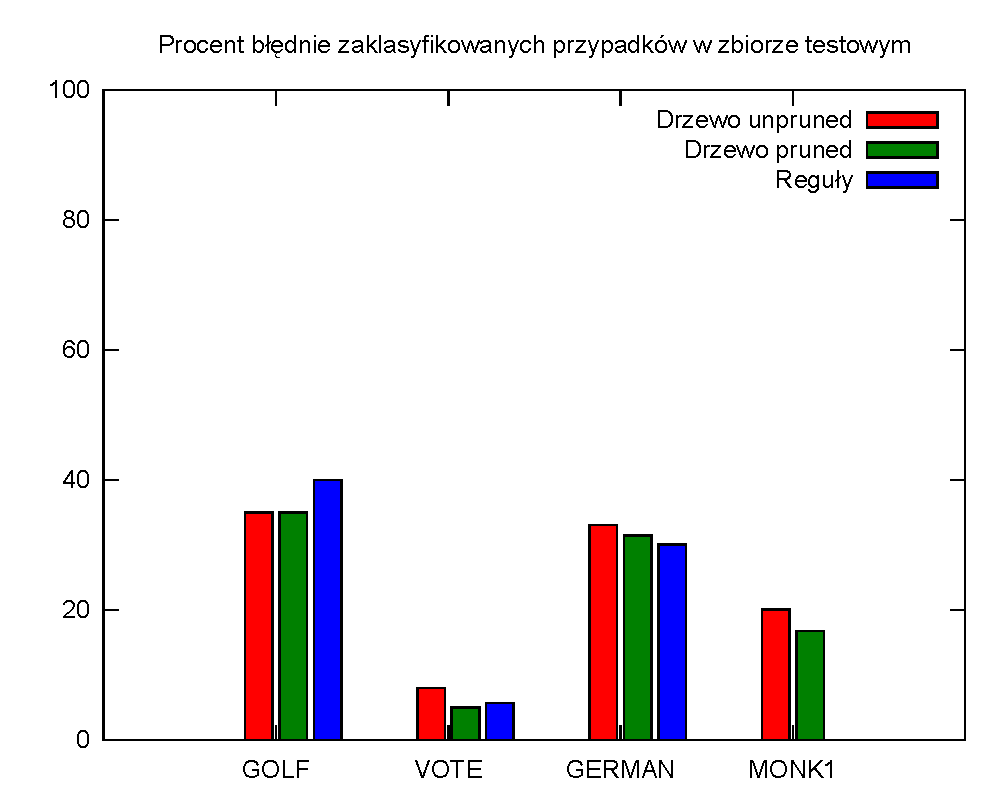
\includegraphics[scale=0.7]{gnuplot/compare-errors.pdf} 
	\caption{Błędy klasyfikowania na zbiorze testującym.}
	\label{p2t2-compare-errors}
\end{figure}

	
\item Przeprowadzając kilka eksperymentów uczenia i~testowania przeanalizuj wpływ parametrów \emph{Confidence Level} i~\emph{Redundancy Factor} na~otrzymywany zbiór reguł.
\end{itemize}

\subsection{Generowanie reguł z~użyciem algorytmu \emph{LEM}}

\begin{itemize}
\item Wygeneruj reguły dla zbioru \emph{HPAP.ISF}.
\item Przyjrzyj się regułom możliwym; opisz je i~,,wydedukuj'', skąd się wzięły.
\end{itemize}

\subsection{Porównanie reguł generowanych za~pomocą algorytmu \emph{LEM} i~\emph{C4.5}}

\begin{itemize}
\item Wygeneruj reguły przy użyciu obu podejść dla zbiorów: \emph{HPAP}, \emph{VOTE} i~\emph{MONK}.
\item Przyjrzyj się niezależnie regułom pewnym i~możliwym (\emph{LEM}).
\end{itemize}

%Dla chętnych:
%\subsection{Przeprowadź eksperyment generowania i~testowania reguł LEM w~ramach cross validation}